\PassOptionsToPackage{unicode=true}{hyperref} % options for packages loaded elsewhere
\PassOptionsToPackage{hyphens}{url}
%
\documentclass[]{scrreprt}
\usepackage{lmodern}
\usepackage{amssymb,amsmath}
\usepackage{ifxetex,ifluatex}
\usepackage{fixltx2e} % provides \textsubscript
\ifnum 0\ifxetex 1\fi\ifluatex 1\fi=0 % if pdftex
  \usepackage[T1]{fontenc}
  \usepackage[utf8]{inputenc}
  \usepackage{textcomp} % provides euro and other symbols
\else % if luatex or xelatex
  \usepackage{unicode-math}
  \defaultfontfeatures{Ligatures=TeX,Scale=MatchLowercase}
\fi
% use upquote if available, for straight quotes in verbatim environments
\IfFileExists{upquote.sty}{\usepackage{upquote}}{}
% use microtype if available
\IfFileExists{microtype.sty}{%
\usepackage[]{microtype}
\UseMicrotypeSet[protrusion]{basicmath} % disable protrusion for tt fonts
}{}
\IfFileExists{parskip.sty}{%
\usepackage{parskip}
}{% else
\setlength{\parindent}{0pt}
\setlength{\parskip}{6pt plus 2pt minus 1pt}
}
\usepackage{hyperref}
\hypersetup{
            pdftitle={Biomechanical Profile},
            pdfborder={0 0 0},
            breaklinks=true}
\urlstyle{same}  % don't use monospace font for urls
\usepackage{longtable,booktabs}
% Fix footnotes in tables (requires footnote package)
\IfFileExists{footnote.sty}{\usepackage{footnote}\makesavenoteenv{longtable}}{}
\usepackage{graphicx,grffile}
\makeatletter
\def\maxwidth{\ifdim\Gin@nat@width>\linewidth\linewidth\else\Gin@nat@width\fi}
\def\maxheight{\ifdim\Gin@nat@height>\textheight\textheight\else\Gin@nat@height\fi}
\makeatother
% Scale images if necessary, so that they will not overflow the page
% margins by default, and it is still possible to overwrite the defaults
% using explicit options in \includegraphics[width, height, ...]{}
\setkeys{Gin}{width=\maxwidth,height=\maxheight,keepaspectratio}
\setlength{\emergencystretch}{3em}  % prevent overfull lines
\providecommand{\tightlist}{%
  \setlength{\itemsep}{0pt}\setlength{\parskip}{0pt}}
\setcounter{secnumdepth}{5}

% set default figure placement to htbp
\makeatletter
\def\fps@figure{htbp}
\makeatother

\RequirePackage{silence}
\WarningFilter{titlesec}{Non standard sectioning command}
\WarningFilter{scrreprt}{Usage of package}
\WarningFilter{scrreprt}{Activating an ugly workaround}
\newcommand{\thesisTheme}{sund} % to colortheme and titlepage image
\usepackage{booktabs}
\usepackage{gensymb}
\usepackage[					% UCPH thesis style
    figuresep=colon,        
    sansserif=false,        
    hangfigurecaption=false,
    hangsection=true,       
    hangsubsection=true,    
    colorize=full,          
    colortheme={\thesisTheme},  % ucph, sund, science, hum, etc.?
    bibsys=biber,
    bibfile=book,       % defines your .bib file
    bibstyle=authoryear,        % refer to https://bit.ly/2YsvIJz
]{ucph}
\usepackage{booktabs}
\usepackage{longtable}
\usepackage{array}
\usepackage{multirow}
\usepackage{wrapfig}
\usepackage{float}
\usepackage{colortbl}
\usepackage{pdflscape}
\usepackage{tabu}
\usepackage{threeparttable}
\usepackage{threeparttablex}
\usepackage[normalem]{ulem}
\usepackage{makecell}
\usepackage{xcolor}
\usepackage[]{biblatex}
\addbibresource{book.bib}
\addbibresource{packages.bib}

\title{Biomechanical Profile}
\author{}
\date{\vspace{-2.5em}}

\begin{document}
\maketitle

{
\setcounter{tocdepth}{1}
\tableofcontents
}
\hypertarget{part-introduction}{%
\part{Introduction}\label{part-introduction}}

\hypertarget{cover-page}{%
\chapter*{Cover page}\label{cover-page}}
\addcontentsline{toc}{chapter}{Cover page}

by Mikkel Roald-Arbøl
2020-06-02

\hypertarget{what-is-biomechanical-profiling}{%
\chapter*{What is Biomechanical Profiling?}\label{what-is-biomechanical-profiling}}
\addcontentsline{toc}{chapter}{What is Biomechanical Profiling?}

When designing training programs coaches face the hard decisions of which physical and technical qualities to prioritize. These decisions are often based on experience, intuition and indirect tests. That's where we come in. \textbf{\emph{At the SportsMechanist our mission is to provide coaches and athletes with valuable information, taking the guess-work out of decision making}}.

\begin{center}\rule{0.5\linewidth}{0.5pt}\end{center}

In short, biomechanical profiling is the quantification of sporting technique.
Biomechanical profiles offer objective sports-specific markers to evaluate athletes' strengths, weaknesses and development, using laws of mechanics.

This report contains three main parts:

\begin{enumerate}
\def\labelenumi{\arabic{enumi}.}
\tightlist
\item
  Background
\item
  Results
\item
  Conclusion
\end{enumerate}

\textbf{Background}. The background section provides a throrough scientific review of the triple jump. A good general understanding of the triple is expected, however all readers are encouraged to read it as it provides the scientific basis for the report.

\textbf{Results}. The results section is the backbone of the profile as it provides measures on the selected markers. These are complemented with \emph{commentaries}, providing an expert interpretation of the results.

\textbf{Conclusion}. The results are taken together, discussed and finally technical recommendations are provided.

\hypertarget{part-background}{%
\part{Background}\label{part-background}}

\hypertarget{triple-jump}{%
\chapter{Triple Jump}\label{triple-jump}}

The triple jump is one of the most demanding sporting disciplines. It consists of three consecutive jumps: a hop, step and jump. The peak ground reaction forces are the highest recorded in \emph{any human movement}, reaching upwards of 21 times bodyweight in the step \autocite{Hay1993}. On top of this, the athlete still has another take-off left. That is why proper technical execution is imperative to a succesful triple jump. Here we will provide a short overview of the most important biomechanical aspects of the triple jump.

Over the years, some research into the biomechanics of the triple jump has been done, mostly during the 80's and 90's. In addition to these there has been published a number of biomechanical reports from various World Championships over the years \autocites{Hommel2009}{Bae2011}{Tucker2017}{Tucker2019} which provides reference values for world class performances. This body of research has been directed in a number of directions:

\begin{enumerate}
\def\labelenumi{\arabic{enumi}.}
\tightlist
\item
  Phase ratio \autocites{Allen2013}{Allen2016a}{Hay1999}{Yu1996}{Hay1992}
\item
  Velocities \autocites{Bayraktar2017}{Liu2015}{Fukashiro1981}
\item
  Take-off leg mechanics \autocites{Perttunen2000}{Ramey1985}{Hay1993}{Fukashiro1981}{Dziewiecki2013}{Dziewiecki2014}
\item
  Free limb mechanics \autocites{Yu1998}{Allen2010}
\item
  Balance
\end{enumerate}

Along with each section, we define a set of \emph{Key performance indicators (KPIs)}. KPIs are the most important variables predicting performance. These differ from sport to sport, and not all are intuitive. At the SportsMechanist we've selected the most appropriate KPIs based on scientific literature and biomechanical reports from World Championships. ~

\clearpage

\hypertarget{phase-ratio}{%
\section{Phase ratio}\label{phase-ratio}}

The phase ratio is the length of each phase relative to the total length of the triple jump (e.g.~35\%, 30\%, 35\%). Three techniques have been described \autocite{Hay1992}:

\begin{itemize}
\tightlist
\item
  \emph{Hop-dominant}: the hop distance is at least 2\% greater than the next largest phase distance.
\item
  \emph{Jump-dominant}: the jump distance is at least 2\% greater than the next largest phase distance.
\item
  \emph{Balanced}: the longest phase distance is less than 2\% greater than the next largest phase distance.
\end{itemize}

As most variables change with technique, this is the first step of an analysis and results should be viewed in light of the technique \autocite{Hay1992}. Whereas the hop-dominant technique used to be favoured, in recent years athletes have transitioned to more balanced and jump-dominant techniques \autocites[e.g.][]{Hay1992}{Tucker2019}.
Trying to determine the \emph{optimal} phase ratio has received much scientific attention. It has been suggested that an optimal phase ratio could be dependent on strength levels or the ability to convert horizontal velocity to vertical velocity \autocites{Allen2013}{Allen2016}{Liu2012}. Although no single optimal distribution has been found, a conservative picture emerges that \emph{no phase should exceed 39\% or be less than 27\% approximately}.~

\begin{longtable}[t]{>{\raggedright\arraybackslash}p{10em}|>{\raggedright\arraybackslash}p{20em}}
\caption{\label{tab:phase-ratio-desc}Phase ratio KPIs}\\
\hline
Variable & Description\\
\hline
Effective distance & Absolute step length for the hop, step and jump in meters.\\
\hline
Relative distance & Relative step length for the hop, step and jump in percents.\\
\hline
Technique & Whether the technique is hop-dominant, jump-dominant or balanced.\\
\hline
\end{longtable}

\clearpage

\hypertarget{velocities}{%
\section{Velocities}\label{velocities}}

\emph{Horizontal velocity.} It has repeatedly been established that \emph{the single best predictor of performance is the horizontal velocity in the run-up}, as up to 94\% of the results can be attributed to run-up velocity \autocites{Fukashiro1981}{Bayraktar2017}{Liu2015}. Interestingly, run-up horizontal velocity is a better predictor of performance than horizontal velocity at take-off \autocite{Bayraktar2017}. This is potentially because the run-up velocity determines the amount of mechanical energy the athlete will be able to produce in the take-off \autocite{Fukashiro1981}. ~

\emph{Take-off angle.} The take-off angle is the product of the horizontal and vertical take-off velocity, and as such is determined by their combination. The take-off angle is typically highest in the jump, however this naturally differ with technique. Thus, hop-dominant jumpers tend to reach higher take-off angles in the hop and jump-dominant jumpers reach higher angles in the jump. ~

\emph{Velocity conversion.} At each take-off vertical velocity is produced at the expense of horizontal velocity. How well a jumper performs this velocity conversion (minimise the loss of horizontal velocity) has been speculated to influence the optimal phase ratio \autocites{Liu2012}{Yu1996}. However, as the current way of quantifying the velocity conversion requires multiple recorded jumps we cannot as of now provide a measure of this in the profile. ~

\begin{table}[!h]

\caption{\label{tab:velocity-desc}Velocities KPIs}
\centering
\begin{tabular}[t]{>{\raggedright\arraybackslash}p{15em}|l}
\hline
Variable & Description\\
\hline
Horizontal velocity & Horizontal velocity at take-off for the hop, step and jump in m/s\\
\hline
Vertical velocity & Vertical velocity at take-off for the hop, step and jump in m/s\\
\hline
Take-off angle & Take-off angle relative to horizontal\\
\hline
\end{tabular}
\end{table}

\clearpage

\hypertarget{take-off-leg-mechanics}{%
\section{Take-off leg mechanics}\label{take-off-leg-mechanics}}

As the triple jump consists of three consecutive take-offs, take-off mechanics are crucial.

\emph{Footstrike}. Two types of footstrike motions have been advocated over time \autocite{Koh1990}. One school advocates an \emph{active landing}, a back-sweeping, pawing motion of the foot. This type of take-off has been described in elite jumpers as early as 1961 by Verhoshanski, and minimises the breaking forces, thus minimizing the loss of horizontal velocity. On the other hand it has been suggested that triple jumpers may benefit from a \emph{blocking landing} in the jump to gain vertical velocity.
The way the footstrike motion is quantified is the velocity of the take-off foot relative to the jumpers center of mass just before the foot contacts the ground. To second the observations by Miller \& Hay \autocite{Miller1986} it can also be noted that all jumpers at major championships have slower foot velocities in the jump than in the prior phases \autocites{Hommel2009}{Tucker2017}{Tucker2019}. ~

\emph{Contact time}. Contact times are often reported, however they are a double edged sword. Shorter contact times are correlated with longer jumps, however the relationship is not as straightforward as that. Contact times in the triple jump is mainly thought to be a consequence of horizontal velocity. The faster the velocity, the shorter time the jumper has on the ground before having to take-off again. So what seems a correlation between contact times and result is in fact correlation between horizontal velocity and result.
Indeed, it is the target for the jumper to exert the greatest amount of force (impulse) on the ground, and following the impulse equation \(F*t=m*v\) either increasing the amount of force \textbf{OR} time will increase the velocity of the jumper. As noted by \textcite{Hay1992}, the consequence is that shorter contact times alone are not desirable. As they are reported at every major championship, we provide these measures, but refrain from commenting on them. ~

\begin{longtable}[t]{>{\raggedright\arraybackslash}p{15em}|l}
\caption{\label{tab:takeoff-desc}Take-off leg KPIs}\\
\hline
Variable & Description\\
\hline
Contact time & Contact time in seconds\\
\hline
Flight time & Flight time in seconds\\
\hline
Absolute foot horizontal velocity & The horizontal velocity of the take-off foot just prior to ground contact. Velocity is relative to the ground.\\
\hline
Relative foot horizontal velocity & The horizontal velocity of the take-off foot just prior to ground contact. Velocity is relative to the CoM.\\
\hline
Knee angle & Minimal knee angle during contact\\
\hline
\end{longtable}

\clearpage

\hypertarget{free-limb-mechanics}{%
\section{Free limb mechanics}\label{free-limb-mechanics}}

\emph{Arm swing.} The free limbs are considered to be the arms and the leg not touching the ground during a contact phase. Especially the arm swing has been the subject of much attention. Yu and Andrews \autocite{Yu1998} found that the arm swing contributes mainly in increasing the vertical velocity and possibly in maintaining balance (definition by \textcite{Hay1993}), whilst decreasing horizontal velocity. However, there exists different arm swing techniques - a topic which has almost not been investigated. The different types of arm swings are: 1) The single arm, 2) the double arm and 3) the arm-and-a-half technique. These have all been utilized at world-class level and have been combined in different ways (e.g.~hop:single arm, step:double arm, jump:double arm). A modelling experiment has suggested that the double-arm swing is benefitial \autocite{Allen2010}, however more work needs to be done before conclusions can be drawn. It is interesting though, that almost all finalists in the 2017 World Championships, nearly all male triple jumpers employed a double-arm swing, whereas all females used a single-arm technique. ~

\emph{Free leg}.

\begin{table}

\caption{\label{tab:free-limb-desc}Free limb KPIs}
\centering
\begin{tabular}[t]{>{\raggedright\arraybackslash}p{15em}|l}
\hline
Variable & Description\\
\hline
Thigh angle & Thigh angle at take-off relative to horizontal\\
\hline
Thigh velocity & Mean angular velocity of thigh of the swing\\
\hline
\end{tabular}
\end{table}

\clearpage

\hypertarget{balance}{%
\section{Balance}\label{balance}}

Balance is a concept familiar to most coaches, however the biomechanical definition is less clear. Hay \autocite{Hay1993} describes it as such:

\begin{quote}
``Balance is a state in which the angular impulse exerted about each of the principal axes of a human body is consistent with the change in angular momentum required about that axis.''
\end{quote}

This statement tells us that angular momentum is at the center of balance. And although.

Many coaches emphasize the importance of upright posture and trunk angle is also reported in WC biomechanical analyses \autocites{Hommel2009}{Tucker2017}{Tucker2019}. So although there are no scientific reports regarding trunk angles, we have included these in our report.

\begin{table}

\caption{\label{tab:balance-desc}Balance KPIs}
\centering
\begin{tabular}[t]{>{\raggedright\arraybackslash}p{15em}|l}
\hline
Variable & Description\\
\hline
Trunk lean angle & Trunk lean angle\\
\hline
Body inclination angle & Body inclination angle\\
\hline
\end{tabular}
\end{table}

\clearpage

\hypertarget{kpi-overview}{%
\chapter{KPI Overview}\label{kpi-overview}}

\begin{table}[!h]

\caption{\label{tab:kpi-overview}Overview of KPIs}
\centering
\begin{tabular}[t]{>{\raggedright\arraybackslash}p{15em}|l}
\hline
Variable & Description\\
\hline
\multicolumn{2}{l}{\textbf{Phase ratio}}\\
\hline
\hspace{1em}Effective distance & Absolute step length for the hop, step and jump in meters.\\
\hline
\hspace{1em}Relative distance & Relative step length for the hop, step and jump in percents.\\
\hline
\hspace{1em}Technique & Whether the technique is hop-dominant, jump-dominant or balanced.\\
\hline
\multicolumn{2}{l}{\textbf{Velocities}}\\
\hline
\hspace{1em}Horizontal velocity & Horizontal velocity at take-off for the hop, step and jump in m/s\\
\hline
\hspace{1em}Vertical velocity & Vertical velocity at take-off for the hop, step and jump in m/s\\
\hline
\hspace{1em}Take-off angle & Take-off angle relative to horizontal\\
\hline
\multicolumn{2}{l}{\textbf{Take-off leg}}\\
\hline
\hspace{1em}Contact time & Contact time in seconds\\
\hline
\hspace{1em}Flight time & Flight time in seconds\\
\hline
\hspace{1em}Absolute foot horizontal velocity & The horizontal velocity of the take-off foot just prior to ground contact. Velocity is relative to the ground.\\
\hline
\hspace{1em}Relative foot horizontal velocity & The horizontal velocity of the take-off foot just prior to ground contact. Velocity is relative to the CoM.\\
\hline
\hspace{1em}Knee angle & Minimal knee angle during contact\\
\hline
\multicolumn{2}{l}{\textbf{Free limbs}}\\
\hline
\hspace{1em}Thigh angle & Thigh angle at take-off relative to horizontal\\
\hline
\hspace{1em}Thigh velocity & Mean angular velocity of thigh of the swing\\
\hline
\multicolumn{2}{l}{\textbf{Balance}}\\
\hline
\hspace{1em}Trunk lean angle & Trunk lean angle\\
\hline
\hspace{1em}Body inclination angle & Body inclination angle\\
\hline
\end{tabular}
\end{table}

\hypertarget{part-results}{%
\part{Results}\label{part-results}}

\hypertarget{profile}{%
\chapter{Profile}\label{profile}}

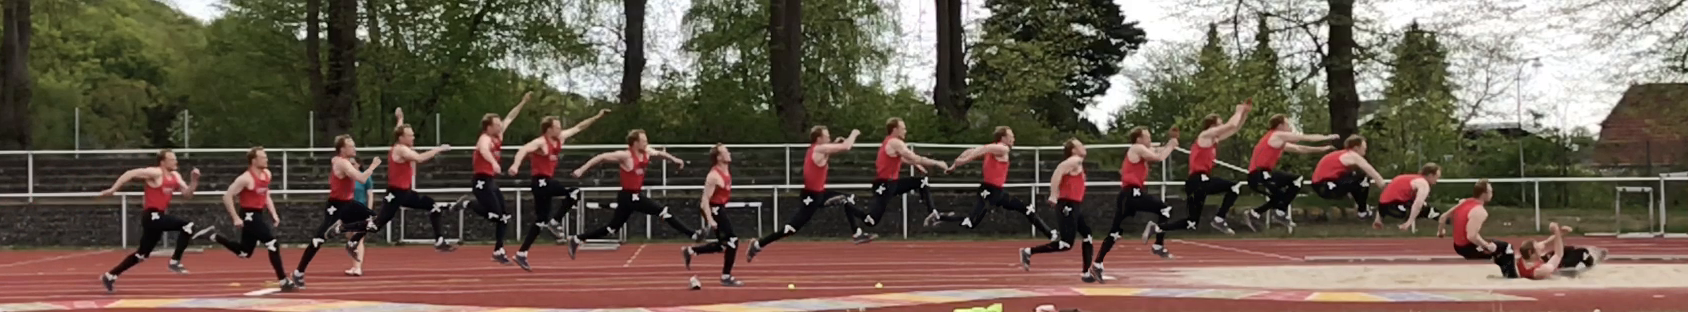
\includegraphics{figures/comp-photo.png} ~

\begin{wraptable}{r}{0pt}
\begin{tabular}{>{\bfseries\raggedright\arraybackslash}p{10em}||>{\raggedright\arraybackslash}p{12em}}
\hline
Name & Jannick Bagge\\
\hline
Age & 26\\
\hline
Bodymass & 78.8 kg\\
\hline
Height & 1.80 m\\
\hline
PB & 15.45 m\\
\hline
Analysed jump & 13.97 m\\
\hline
Date & 10/5/2020\\
\hline
Comment & 10 step approach\\
\hline
\end{tabular}\end{wraptable}

In the results' section we go through each technical component, providing:

\begin{itemize}
\tightlist
\item
  KPIs
\item
  Graphs and plots
\item
  Commentaries
\end{itemize}

\clearpage

\hypertarget{phase-ratio-1}{%
\section{Phase ratio}\label{phase-ratio-1}}

\begin{table}[H]
\centering
\begin{tabular}{l|l|l|l}
\hline
  & Hop & Step & Jump\\
\hline
Relative distance & 36\% & 30\% & 34\%\\
\hline
Effictive distance & 4.99 & 4.10 & 4.71\\
\hline
\end{tabular}
\end{table}

\begin{verbatim}
##                              Technique is Balanced
\end{verbatim}

~

\hypertarget{commentary}{%
\subsection{Commentary}\label{commentary}}

Jannick is employing a balanced technique with a 30\% step phase. The rest of the analysis will be viewed in light of this.

\clearpage

\hypertarget{velocities-1}{%
\section{Velocities}\label{velocities-1}}

\begin{table}[H]
\centering
\begin{tabular}{l|l|l|l}
\hline
  & Hop & Step & Jump\\
\hline
Horizontal velocity & 7.95 & 6.67 & 6.26\\
\hline
Vertical velocity & 2.05 & 2.01 & 2.01\\
\hline
Take-off angle & 14° & 17° & 18°\\
\hline
\end{tabular}
\end{table}

~

\includegraphics{report_files/figure-latex/horizontal velocity-1.pdf}
~

\includegraphics{report_files/figure-latex/vertical velocity-1.pdf}
~

\hypertarget{commentary-1}{%
\subsection{Commentary}\label{commentary-1}}

When looking at the horizontal velocity it is important to remember that the jump is from a short approach, thus velocity is not as high.

Quite a bit of horizontal velocity is lost in the step, whereas the loss is kept very low in the two other take-offs. The vertical velocities are very reasonable, almost comparable to those achieved at world-class level \autocites{Miller1986}{Allen2013}, with the exception of the jump which is not high. It is apparent from the take-off angles that the step is probably too high (with a big loss of horizontal velocity), whereas the jump becomes too shallow.

\begin{center}\rule{0.5\linewidth}{0.5pt}\end{center}

\textbf{Strengths}

\begin{itemize}
\tightlist
\item
  Good maintenance of v\textsubscript{h} in hop and jump
\item
  Ability to produce high v\textsubscript{v}
\end{itemize}

\textbf{Challenges}

\begin{itemize}
\tightlist
\item
  Excessive loss of v\textsubscript{h} in step
\item
  Step too steep
\item
  Jump too shallow
\end{itemize}

\clearpage

\hypertarget{take-off-leg-mechanics-1}{%
\section{Take-off leg mechanics}\label{take-off-leg-mechanics-1}}

\begin{table}[H]
\centering
\begin{tabular}{l|l|l|l}
\hline
  & Hop & Step & Jump\\
\hline
Contact time & 0.12 & 0.15 & 0.17\\
\hline
Flight time & 0.50 & 0.44 & 0.56\\
\hline
Absolute foot horizontal velocity & 2.75 & 2.01 & 1.81\\
\hline
Relative foot horizontal velocity & -5.63 & -5.52 & -4.99\\
\hline
Minimal knee angle & 146° & 129° & 133°\\
\hline
\end{tabular}
\end{table}

~
\includegraphics{report_files/figure-latex/vGRF-1.pdf}
~

\includegraphics{report_files/figure-latex/hGRF-1.pdf}
~

\hypertarget{commentary-2}{%
\subsection{Commentary}\label{commentary-2}}

Again, the step and jump are the phases which demand attention. The vertical forces produced during the hop looks very reasonable. However, it seems excessive for the step and insufficient in the jump - the second peak of the jump GRF doesn't appear.

Jannick employs active landings in all phases at reported world-class level \autocite{Koh1990}.

\begin{center}\rule{0.5\linewidth}{0.5pt}\end{center}

\textbf{Strengths}

\begin{itemize}
\tightlist
\item
  Active landings
\end{itemize}

\textbf{Challenges}

\begin{itemize}
\tightlist
\item
  Excessive vertical force in step
\item
  Insufficient vertical force in jump
\end{itemize}

\clearpage

\hypertarget{free-limb-mechanics-1}{%
\section{Free limb mechanics}\label{free-limb-mechanics-1}}

\begin{table}[H]
\centering
\begin{tabular}{l|l|l|l}
\hline
  & Hop & Step & Jump\\
\hline
Thigh angular velocity & 688°/s & 700°/s & 451°/s\\
\hline
Thigh angle & -9° & -7° & -28°\\
\hline
\end{tabular}
\end{table}

~

\includegraphics{report_files/figure-latex/angular-velocity-1.pdf}
~

\hypertarget{commentary-3}{%
\subsection{Commentary}\label{commentary-3}}

If we turn our attention to the jump, we can really see the lack of swinging speed during the jump! In the graphs we're looking at the negative velocities during support, and neither peak or mean velocities are nowhere near what the were during the hop or step. The performance during hop and step are on level with world-class athletes. Taken together with the fact that the swing ends much further from horizontal, the vertical impulse generated from the free limbs could be much greater.

\begin{center}\rule{0.5\linewidth}{0.5pt}\end{center}

\textbf{Strengths}

\begin{itemize}
\tightlist
\item
  Good thigh velocity in hop and step
\item
  Good thigh angles in hop and step
\end{itemize}

\textbf{Challenges}

\begin{itemize}
\tightlist
\item
  Inadequate thigh velocity in jump
\item
  Low thigh angle in jump
\end{itemize}

\clearpage

\hypertarget{balance-1}{%
\section{Balance}\label{balance-1}}

\begin{table}[H]
\centering
\begin{tabular}{l|l|l|l}
\hline
  & Hop & Step & Jump\\
\hline
Trunk angle at TD & 7° & 1° & 10°\\
\hline
Trunk angle at TO & 14° & 13° & 8°\\
\hline
Inclination angle at TD & -19° & -18° & -17°\\
\hline
Inclination angle at TO & 31° & 33° & 30°\\
\hline
\end{tabular}
\end{table}

~

\hypertarget{commentary-4}{%
\subsection{Commentary}\label{commentary-4}}

The trunk angle suggests that Jannick has a pronounced forward lean, something that could potentially explain the steep step take-off angle, loss of horizontal velocity and eventually the inefficient jump phase.

\begin{center}\rule{0.5\linewidth}{0.5pt}\end{center}

\textbf{Strengths}

\begin{itemize}
\tightlist
\item
  Manages forward rotation
\end{itemize}

\textbf{Challenges}

\begin{itemize}
\tightlist
\item
  Excessive forward lean
\end{itemize}

\clearpage

\hypertarget{kpi-summary}{%
\chapter{KPI Summary}\label{kpi-summary}}

\begin{table}[H]
\centering
\begin{tabular}{l|l|l|l}
\hline
  & Hop & Step & Jump\\
\hline
\multicolumn{4}{l}{\textbf{Phase ratio}}\\
\hline
\hspace{1em}Relative distance & 36\% & 30\% & 34\%\\
\hline
\hspace{1em}Effictive distance & 4.99 & 4.10 & 4.71\\
\hline
\multicolumn{4}{l}{\textbf{Velocities}}\\
\hline
\hspace{1em}Horizontal velocity & 7.95 & 6.67 & 6.26\\
\hline
\hspace{1em}Vertical velocity & 2.05 & 2.01 & 2.01\\
\hline
\hspace{1em}Take-off angle & 14° & 17° & 18°\\
\hline
\multicolumn{4}{l}{\textbf{Take-off leg}}\\
\hline
\hspace{1em}Contact time & 0.12 & 0.15 & 0.17\\
\hline
\hspace{1em}Flight time & 0.50 & 0.44 & 0.56\\
\hline
\hspace{1em}Absolute foot horizontal velocity & 2.75 & 2.01 & 1.81\\
\hline
\hspace{1em}Relative foot horizontal velocity & -5.63 & -5.52 & -4.99\\
\hline
\hspace{1em}Minimal knee angle & 146° & 129° & 133°\\
\hline
\multicolumn{4}{l}{\textbf{Free limbs}}\\
\hline
\hspace{1em}Thigh angular velocity & 688°/s & 700°/s & 451°/s\\
\hline
\hspace{1em}Thigh angle & -9° & -7° & -28°\\
\hline
\multicolumn{4}{l}{\textbf{Balance}}\\
\hline
\hspace{1em}Trunk angle at TD & 7° & 1° & 10°\\
\hline
\hspace{1em}Trunk angle at TO & 14° & 13° & 8°\\
\hline
\hspace{1em}Inclination angle at TD & -19° & -18° & -17°\\
\hline
\hspace{1em}Inclination angle at TO & 31° & 33° & 30°\\
\hline
\end{tabular}
\end{table}

\hypertarget{part-conclusion}{%
\part{Conclusion}\label{part-conclusion}}

\hypertarget{conclusion}{%
\chapter{Conclusion}\label{conclusion}}

\textbf{Primary errors}\\
The analysis highlighted three primary errors:

\begin{enumerate}
\def\labelenumi{\arabic{enumi}.}
\tightlist
\item
  Forward lean
\item
  Steep step
\item
  Inefficient jump
\end{enumerate}

\textbf{Interpretation and discussion}\\
Jannick looses excessive horizontal velocity during especially the step.
The ineffective jump might well be caused by the forward lean.
We were able to tell that in the jump he produces insufficient vertical velocity (and force) and that seems mainly caused by a lack of swinging of the free leg and probably arms. Swinging motions, especially by the arms, have a great effect on the vertical velocity produced at the cost of horizontal velocity \autocite{Yu1998}. However, in the jump this trade-off offers a good deal.

\textbf{Recommendations}\\
In conclusion, we recommend that the technical training focuses on upright posture and achieving greater height in the jump, mainly through improving the active free limb motions.

\begin{center}\rule{0.5\linewidth}{0.5pt}\end{center}

\textbf{Recommendations}

\begin{enumerate}
\def\labelenumi{\arabic{enumi}.}
\tightlist
\item
  Upright posture
\item
  More shallow step, maintaining v\textsubscript{h}
\item
  Steeper jump, with active free limb swinging
\end{enumerate}

\begin{center}\rule{0.5\linewidth}{0.5pt}\end{center}

\textbf{Strengths}

\begin{itemize}
\tightlist
\item
  Balanced technique
\item
  High levels of v\textsubscript{v} production
\item
  Active landings
\end{itemize}

\textbf{Challenges}

\begin{itemize}
\tightlist
\item
  Excessive forward lean
\item
  Steep step
\item
  Excessive loss of v\textsubscript{h} in step
\item
  Shallow jump
\item
  Inadequate swinging motions in jump
\end{itemize}

\clearpage

\printbibliography

\end{document}
